
As seen before in sec \ref{sec:tau_lepton}, when a $\tau$ is produced in a collision, it can decay into several different final states.
Hadronic final states, denoted \tauh, represent about 65\% of tau decays.
In recnstruction phase, Hadronic final states are characterised by 1 or 3 charged hadrons with or without \pizero .

Similar particles can be reconstructed from the final states of QCD jets.
Since those QCD jets greatly outnumber \tauh in the final states of proton-proton collisions at the LHC, \tauh identification algorithms have be designed to reject QCD jets as much as possible while keeping a \tauh identification efficiency somewhere between 35\% and 70\%, depending on the purity needed by an analysis.

Such pre-existing standard CMS identification, as will be presented in section \ref{sec:std_tau_id}, has reached excellent performances thanks to the use of particle-flow reconstruction but does not use its full potential.

Deep learning algorithms, that will be presented in section \ref{sec:NN}, have shown a capacity to use all available information at their disposal in the task they are trained for. More recently, they have started to be used with great results in similar applications as in heavy flavour jet-tagging \cite{btagging_NN}. Some neural network designs, called architectures, specifically designed for high energy physics proton-proton collisions have started to appear too. One of such is the Recursive Neural Network (RecNN) as is detailed in this article \cite{qcd_aware_RecNN}, the section \ref{sec:RecNN} will detail the adaptation to the \tauh identification task and the improvements from the original design.

But first, section \ref{sec:NN_datasets} will give a quick overview of the CMS simulated data that will be used to quantify the performance of both standard and new technique. This simulation will also be used to train the deep learning algorithm

\section{Simulation of QCD jets and hadronic $\tau$ decays}
\label{sec:NN_datasets}

In order to compare signal efficiency and background rejection power, but also to provide a training set for our deep learning algorithm, datasets of QCD jets and hadronic tau decays have been selected from the CMS simulations datasets \ref{sec:cms_physics_event_generation}, as will be detailed in sub-section \ref{sec:NN_datasets_gen} .

To test algorithms in real conditions, reconstructed jets from simulated \tauh and QCD jets will be selected individually from collision-wide simulated collisions.
As seen in sec \ref{sec:cms_physics_event_reconstruction}, after particle-detector interaction is simulated, reconstruction will undergo the exact same algorithms in both real data in simulation, meaning both classical and, if proven to be useful, deep-learning based algorithms identification algorithms, the reconstruction steps that precede identification will be detailed in sub-section \ref{sec:NN_datasets_pf}. Although to be able to quantify both methods in terms of background rejection and signal identification, only simulation will be used to compare.

In order to clearly quantify the previously-mentioned performances, background and signal definitions will be defined in \ref{sec:NN_datasets_s_b_def}.

\subsection{Generator and detector interaction}
\label{sec:NN_datasets_gen}

\begin{table}[ht]
    \centering
    \begin{adjustbox}{max width=\textwidth}
    \begin{tabular}{c||c|c}
        & \tauh (signal) & QCD jets (background) \\
        \hline \hline
        \multirow{3}{*}{Hard processes} & susy ggH to $\tau\tau$ & \multirow{3}{*}{\begin{minipage}{0.4\textwidth}QCD multijets samples ordered by \pt : 15-30, 30-50, 50-80, 80-120, 120-170, 170-300 \end{minipage}} \\
        \cline{2-2}
         & susy bbh to $\tau\tau$ & \\
        \cline{2-2}
         & DY to tautau & \\
        \hline
        phase-space cuts & \multicolumn{2}{c}{$20<\pt<100 abs(\eta)<0.8$}\\
        \hline
        specific extra cuts & matched with gen-level \tauh & any \\
        \hline
    \end{tabular}
    \end{adjustbox}
    \caption{Provenance and cuts applied to reconstructed jets defining signal and background.}
    \label{tab:NN_b_s_diff}
\end{table}

As seen in section \ref{sec:LHC_collision}, collisions in the LHC apparatus can be of different "hard" processes. From those hard processes, only the ones leading to a final state including our main background or signal is of interest. 
In our case only hard processes leading to QCD jets, and our signals most important production modes will be used.
The reconstructed jets have been selected from the hard processes detailed in table \ref{tab:NN_b_s_diff}.

The pp collisions events are generated with PYTHIA 8 \cite{pythia}, and are then processed by the CMS GEANT4 simulation, as is detailed in section \ref{sec:cms_physics_event_generation}.
The generation information is kept and will be labelled as true or gen-level informations.

\subsection{Particle-flow reconstruction and jet clustering}
\label{sec:NN_datasets_pf}
All the information gathered by the CMS detectors detailed in \ref{sec:detectors}, whether form simulation or real data-taking, is fed to particle flow algorithm as is detailed in \ref{sec:pf}.
The particle flow algorithm provides the list of stable particles that have been reconstructed. Higher level objects, such as jets are reconstructed by combining elements from this list using clustering algorithms detailed in \ref{sec:jet_clustering}.
In this case the clustering is done using CMS's anti-kt algorithm with distance parameter R = 0.4.

At this point all reconstructed particles, isolated or not, are part of a reconstructed jet.

\subsection{Signal and background definition}
\label{sec:NN_datasets_s_b_def}

Identification of \tauh is done on each reconstructed jet basis, meaning only elements of a single reconstructed jet are taken into account for this identification. 
Signal and background reconstructed jets are here defined from their hard process origin and some extra cuts to ensure purity.
The cuts can be found in table \ref{tab:NN_b_s_diff} where the matching between reconstructed jets and gen-level \tauh is done by ensuring their proximity, meaning that the distance separating them in the $\eta-\phi$ plane is less than $0.1$.

\section{The standard CMS hadronic $\tau$ decays ID}
\label{sec:std_tau_id}
\subsection{Decay mode finding}

The PF algorithm has so far provided each reconstructed jet with particles that could be \tauh decay products.

The particles are used as input to the hadrons-plus-strip (HPS) algorithm \cite{tauh_reconstruction} to reconstruct and identify PF \tauh candidates. 
This algorithm is seeded by the reconstructed jets of \pt > 14 GeV and $|\eta|$ < 2.5.
The jet constituent particles are combined into \tauh candidates compatible with one of the main $\tau$ decay modes, $\tau^- \rightarrow h^- \nu_\tau$, $\tau^- \rightarrow h^- \pizero \nu_\tau$, $\tau^- \rightarrow h^- \pizero \pizero \nu_\tau$, $\tau^- \rightarrow h^- h^+ h^- \nu_\tau$. The decay mode $\tau^- \rightarrow h^- h^+ h^- \pizero \nu_\tau$ is not considered owing to its relatively small branching fraction and high contamination from quark and gluon jets.

Because of the large amount of material in the tracker \ref{fig:tracker_material}, photons from \pizero decays often convert before reaching the ECAL. The resulting electrons and positrons can be identified as such by the PF algorithm or, in the case their track is not reconstructed, as photons displaced along the $\phi$ direction because of the bending of their trajectory bent by the magnetic field.
Neutral pions are therefore obtained by adding iteratively reconstructed photons and electrons located in a strip of size $0.05 \times 0.20$ in the ($\eta$,$\phi$) plane:

Every reconstructed electrons and photons of $\pt > 0.5 GeV$ in the strip are added iteratively from highest to lowest \pt.
At every step, the position of the center of the strip is re-computed as a \pt-weighted average of the position of all constituents.
Any electron or photon not included in an existing strip is used as seed to another new strip.

\tauh candidates are then formed by creating all combininations of either one or three charged-particle and up to two strips in the jet.
Each \tauh candidate is then required to have a mass compatible with its decay mode and to have unit charge.
Collimated \tauh are selected by requiring all charged hadrons and neutral pions to be within a circle of radius $\Delta R = (2.8 GeV)/\pt$ in the ($\eta$,$\phi$) called the signal cone.
The size of the signal cone is, however, not allowed to increase above 0.1 at low \pt, nor to decrease below 0.05 at high \pt. It decreases with \pt to account for the boost of the $\tau$ decay products. Finally, the highest \pt selected \tauh candidate in the jet is retained. The four-momentum of the \tauh candidate is determined by summing the four-momenta of its constituent particles.
More precisions on requirements and hypothesis can be found in \cite{tauh_reconstruction}.

\subsection{Isolation}


\tauh candidates reconstructed from QCD jets are likely to be surrounded by other particles coming from the hadronization of quarks and gluons.
Isolation therefore can be useful to reject a lot of background QCD jets.

Two approaches are available : cut-based and multi-variate
Cut-based : 
\begin{itemize}
    \item Isolation is roughly the sum of \pt of charged particles and photons with $\pt > 0.5$ GeV within an isolation cone of dR=0.5 centered around the \tauh direction, excluding particles used to form the \tauh candidate.
    \item In order to mitigate pileup contribution, tracks associated to considered charged particles are required to be compatible with the \tauh production vertex within a distance $\Delta z < 0.2 cm$ and $\Delta r < 0.03 cm$.
\begin{equation}
    I_{\tau} = \sum_{charged, \Delta z<0.2 cm} \pt + max \Big\{ 0, \sum_{\gamma} \pt - \Delta\beta \Big\}
    \label{eq:isolation}
\end{equation}
\begin{equation}
    \Delta \beta = 0.46 \sum_{charged,\Delta z>0.2 cm} \pt
\end{equation}
    \item Working points are defined by the thresholds on the value taken by the isolation defined in equation \ref{eq:isolation}. Usual working points such as Loose, medium, tight are thresholds are 2.0, 1.0 and 0.8 GeV respectively.
\end{itemize}

Multi-variate : BDT based
\begin{itemize}
    \item Decision trees are a machine learning technique that relies on finding the best successive cuts on the chosen variables to separate signal and background in a training set.
    \item Boosting is a method of combining many weakly classifying trees into a strong classifier.
    \item A BDT is trained on an appropriate choice of isolation variables to give best separation between QCD jets and \tauh : 
    \begin{itemize}
        \item charged- and neutral-particle isolation sums defined as in eq \ref{eq:isolation}.
        \item The reconstructed decay mode.
        \item the transverse impact parameter $d_0$ of the leading tack of the \tauh candidate and its significance $d_0 / \sigma_{d_0}$
        \item the distance between the $\tau$ production and decay vertices, $|\Vec{r}_{SV} - \Vec{r}_{PV}|$, and its significance $|\Vec{r}_{SV} - \Vec{r}_{PV}|/\sigma_{|\Vec{r}_{SV} - \Vec{r}_{PV}|}$, along with a flag indicating wether a decay vertex has successfully been reconstructed for a given \tauh candidate. The positions of the vertices, $\Vec{r}_SV$ and $\Vec{r}_PV$, are reconstructed using the adaptive vertex fitter algorithm \cite{Waltenberger_2007}.
    \end{itemize}
    \item More details in \cite{tauh_reconstruction}.
\end{itemize}

\subsection{Anti-leptons discriminants}

\tauh can also be wrongly reconstructed from electrons and muons, particularly in the $h^{\pm}$ decay mode. Electrons radiating a bremsstrahlung photon that subsequently converts may also get reconstructed in the $h^{\pm}\pizero$ decay mode. Therefore discriminants have been developed to separate such leptons from \tauh.

Electrons are discriminated by a BDT using observables that quantify the distribution in energy depositions in the ECAL, in combination with observables sensitive to the amount of bremsstrahlung emitted along the leading track, and observables sensitive to the overall particle multiplicity, to distinguish electromagnetic from hadronic showers.
All those variables are listed in \cite{tauh_reconstruction}.
    
Muons are rejected from \tauh candidates by requiring that no track segments are found in at least two muon stations within a cone of size $\Delta R = 0.3$ around the \tauh direction. \tauh candidates are also rejected when the sum of the energies in the ECAL and HCAL corresponds to les than 20\% of the momentum of their leading track.
    % \item Electrons are discriminated with a BDT using the following variables:
    % \begin{itemize}
    %     \item Electromagnetic energy fraction of the charged particles and photons that constitue the \tauh candidate : $E_{ECAL}/(E_{ECAL} + E_{HCAL})$.
    %     \item $E_{ECAL}/p$ and $E_{HCAL}/p$, defined as rations of ECAL and HCAL energies relative to the momentum of the leading charged-particle track of the \tauh candidate.
    %     \item $\sqrt{\sum(\Delta \eta)^2 \pt^{\gamma}}$ and $\sqrt{\sum(\Delta \phi)^2 \pt^{\gamma}}$, the respective \pt-weighted (in GeV) root-mean-square distances in $\eta$ and $\phi$ between the photons in any strip and the leading charged particle.
    %     \item $\sum E_{\gamma}/E_{\tau}$, the fraction of \tauh energy carried by photons.
    %     \item $F_{brem} = (p_{in}-p_{out})/p_{in}$, where $p_{in}$ and $p_{out}$ are measured by the curvature of the leading track, reconstructed using the GSF algorithm, at the innermost and outermost positions of the tracker.
    %     \item $(E_e + \sum E_{\gamma})/ p_{in}$, the ratio between the total ECAL energy and the ineer track momentum. Thr quantities $E_e$ and $E_{\gamma}$ represent the energies of the electron cluster and of bremsstrahlung photons, respectively. $\sum E_{gamma}$ is reconstructed by summin the energy depositions in ECAL clusters located along the tangent to the GSF track.
    %     \item $\sum E_{\gamma}/(p_{in}-p_{out})$, the ratio of energies of the bremsstrahlung photons measured in the ECAL and in the tracker.
    %     \item $m_{\tauh}$, the mass of the \tauh candidate.
    %     \item $$
    % \end{itemize}

\subsection{Performance}

Receiver Operating Characteristic (ROC) curves are an efficient tool to visualize and compare the performances of different approaches. These curves are built by computing the signal efficiency and background rejection on different working point of a given approach. Each working point is then a point of the curve in the signal efficiency vs background rejection space.
Generally, a numerical figure of merit is the area under the ROC curve, called ROC AUC, as it is maximum when signal efficiency and background rejection is perfect.
In our case, ROC AUC might not be the best figure of merit, as it treats the background rejection and signal efficiency with the same relative importance.
Indeed in our case QCD jets are overwhelmingly more present in collisions than \tauh, meaning useful working points must be in the region of high background rejection.

\subsection{Intrinsic limitations}

All those identification methods rely heavily on either designing variables that are likely to have discriminating power, such as isolation, or the many variables used by the BDTs. Those variable potentially do not take into account other information that have been gathered in the detection and reconstruction.
Fine tuning the choice of variable by hand could be a tedious process, as many studies would be needed and the possibilities of information combinations are infinite. This is why machine learning algorithms such as BDTs have been used, as those algorithms are able to come up with a finer tuned variable, their output, by learning how to combine the available information.
An intrinsic limit of such algorithms comes in the information that is available in the given set of inputs. 
A possible improvement should therefore be expected from using a more complete set of variable rather than a chosen set.


\section{From a single neuron to recurrent networks}
\label{sec:NN}
Neural networks have gained some steam lately in fields such as big data, image recognition and even pseudo-data generation.
They are good in performing tasks where a lot of data with truth are available, such as fields with good existing simulation.
Based on basic understanding of a human neuron and using the exponential possibilities of combining such neurons together.
Such combination can be designed to be adapted to the task at hand and are called architectures.
Some architectures have been developed to be able to take a non pre-defined number of variables, such as the recurrent neural networks, originally developed in language processing.

\subsection{Basics : neurons, dense networks, deep learning}

\subsubsection{Neuron}

\begin{figure}
    \centering
    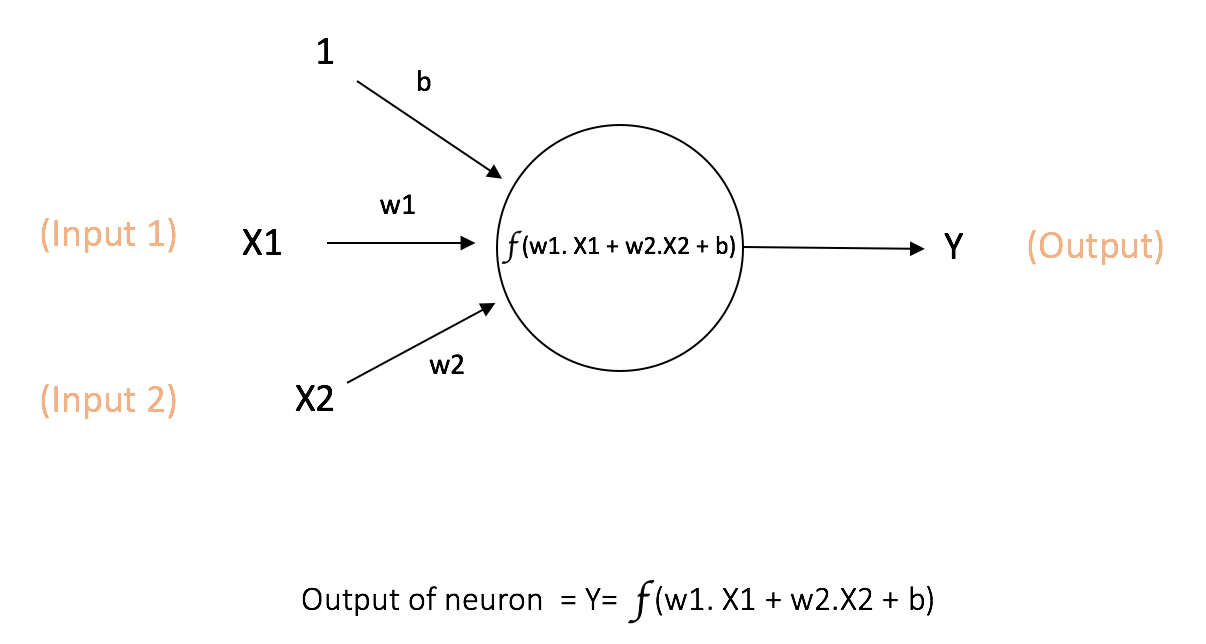
\includegraphics[width=0.8\textwidth]{Images/neuron_diagram}
    \caption{Diagram of a single neuron}
    \label{fig:neuron_diagram}
\end{figure}


\begin{figure}
    \centering
    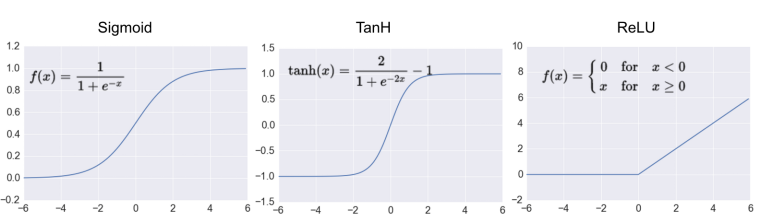
\includegraphics[width=\textwidth]{Images/activation_functions.png}
    \caption{Some activation functions and their visualisation.}
    \label{fig:activation_functions}
\end{figure}

As can be seen in: \ref{fig:neuron_diagram}, a neuron takes several inputs, weighs each of them with its own set of weights, then adds the weighted inputs together with a bias.
This total is now given as input to an activation function. 
The output of the activation function is now the output of the neuron.
There are several kinds of activation functions. Those activation need to be nonlinear functions and also need to be differentiable for reasons that will be detailed once the network and backpropagation methods are explained later.
Examples of mainly used activation functions in \ref{fig:activation_functions}


\subsubsection{Densely connected network}


\begin{figure}
    \centering
    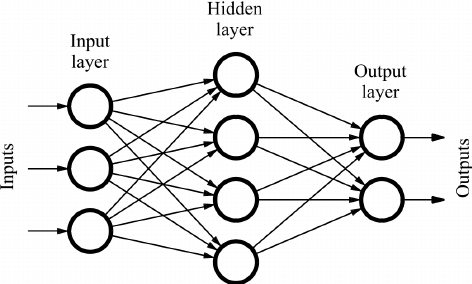
\includegraphics[width=0.5\textwidth]{Images/dense_network.png}
    \caption{Diagram of an example of a feed-forward densely connected network with 3 input variables, 4 neurons in the hidden layer and 2 output neurons.}
    \label{fig:dense_network}
\end{figure}

A network can be created by organising neurons such as a neuron's input is another neuron's output.
For now we will focus on a simple case : the feed-forward densely connected network.
Feed forward means that there is no cycle in the propagation of the evaluation from inputs to outputs.
In this architecture, neurons are organised by layers, with each neuron's output being an input to each neuron in the next layer as seen on \ref{fig:dense_network}.
The Universal approximation theorem states that a network of non-linearly activated neurons can approximate continuous functions on compact subsets of ${\rm I\!R}^{n}$ for width-$n$ networks. Hence why the non-linear activation function.

\subsubsection{Loss function and backpropagation}

The goal now is to change weights and biases of the network so that the ouput will be as correlated as possible with the chosen task.
This will be done in a training phase, in which the task's completion of the network can be compared to the truth on a set of inputs.
The training phase's goal will be to give outputs as close as possible to the truth.
First a metric is defined to tell how close the network output is to the desired output.
This metric will be chosen to be minimum when the output of the network is exactly the desired output.
This function is called loss function.
In order to avoid stagnation from contradicting learning in different examples, before each adaptation of the network, the loss function will be averaged over several training.
There are several optimizers algorithms that allows to modify the weights in order to minimize the loss function.
Those optimizers's secondary goal is to avoid getting stuck in networks configurations that stay in a local minima of the loss function.
To avoid this, momentum based optimizers have been used, those optimizers are going to base the changes in the network on previous states of the loss functions. 
Another problem common in neural network training is vanishing gradient. This problem arises because a weight update is proportional to the partial derivative of the loss function with respect to the activation of later layers. 
Since activation function have "flat" regions, the partial derivative of the loss function can then be very small, effectively preventing the weight from changing its value.
To avoid this one can use activation functions such as ReLU, which is less likely to be stuck in a "flat" region of its activation. Also the use of the cross-entropy loss function allows certain terms to cancel in the backpropagation, avoiding such cases.
One final possibility is to avoid the feed-forward architecture overall, as the vanishing gradient problem is exponentially more problematic with the "depth" of a network. An example of such an architecture will be detailed in the next section.
    % \begin{equation}
    %     L = \frac{1}{n} \sum_x L_x
    % \end{equation}
    % \item (base explanation same way as http://neuralnetworksanddeeplearning.com/chap2.html and cite!)
    % \item notation : 
    % \begin{itemize}
    %     \item $w_{jk}^{l}$  denote the weight for the connection from the $k^{th}$ neuron in  the $(l-1)^{th}$ layer to the $j^{th}$ neuron in the $l^{th}$ layer and $b_{j}^{l}$ the bias of the $j^{th}$ neuron in the $l^{th}$ layer
    %     \item $\sigma$ is the activation unction
    %     \item $a_{j}^{l}$ is the activation of the $j^{th}$ neuron in the $l^{th}$ layer
    %     \item therefore 
    %     \begin{equation}
    %         a_{j}^{l} = \sigma \Big( \sum_k w_{jk}^{k}a_{k}^{l-1} + b_{j}^{l} \Big)
    %     \end{equation}
    %     \item to lighten the scripture, let's use the vectorized form:
    %     \begin{equation}
    %         a^l = \sigma \Big( w^l a^{l-1} + b^l \Big)
    %     \end{equation}
    %     \item with
    %     \begin{equation}
    %         f\begin{pmatrix} x_1 \\ x_2 \end{pmatrix} = \begin{pmatrix} f(x_1) \\ f(x_2) \end{pmatrix}
    %     \end{equation}
    %     \item also to lighten the scripture let's define :
    %     \begin{equation}
    %         z_j^l = \sum_k w^l_{jk} a_k^{l-1} + b_j^l
    %     \end{equation}
    %     \item and
    %     \begin{equation}
    %         (s \odot t)_j = s_j t_j
    %     \end{equation}
    %     \item now let's define the "learnability" (good word?) of neuron $j$ in the $l^th$ layer:
    %     \begin{equation}
    %         \delta_j^l \equiv \frac{\partial L}{\partial z_l^j}
    %     \end{equation}
    % \end{itemize}
    % \item problem : local minimas
    % \item part of the solution : momentum
    % \item further solution : ADAM
    % \item problem : vanishing gradient
    % \item part of the solution : right choice of loss function (cross-entropy)


\subsection{Recurrent neural networks}

\begin{figure}
    \centering
    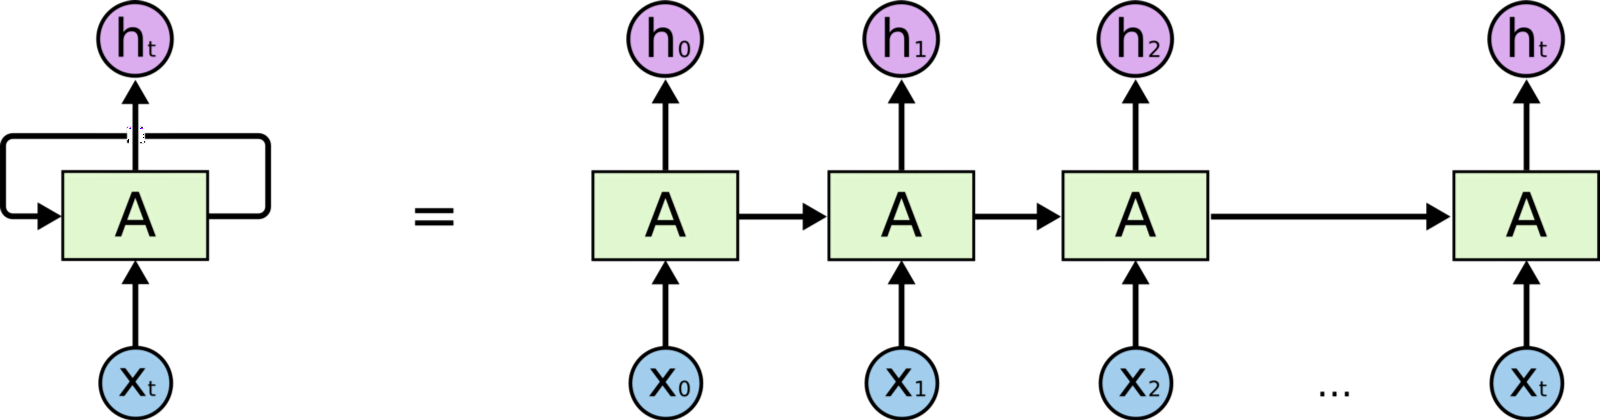
\includegraphics[width=\textwidth]{Images/recurrent_network.png}
    \caption{Diagram of the evaluation of a recurrent network on successive sets of inputs}
    \label{fig:recurrent_network}
\end{figure}

The architecture of a neural network should be chosen to either accommodate the context of the task, or to minimize the need of a sizeable training sample.
With this in mind lots of different architecture have been developed.
One such architecture has been mainly optimised for language process, in which the number of words in a sentence is not pre-defined.
The idea is to have the same block of layers to be evaluated on each entry, while each evaluation gives an secondary output that will be used as a secondary input to the next evaluation . see \ref{fig:recurrent_network}
One can understand the communication between successive evaluation as an "inner representation", and the outputs at each evaluation an "partial output" that the network would give using only the information gathered at this stage.
(gradient descent avoided if "inner representation" doesn't go through a layer) (careful this isn't True with recursive)
This architecture already creates a strong argument to our case as the reconstructed jet could be the sentence and particles the words.

\section{Recursive neural network}
\label{sec:RecNN}
As we have seen, architecture that could process different number of entries as the RNN exist
Will be useful for particle-level jet processing as the number of particle changes from one jet to the other.
Now we could also tune an architecture to be even more pertinent to the situation.
All reconstructed particle come from either hadronisation or decay of particles.
Similar problem was explored in (REF GILLES PAPER HERE) QCD-aware recursive architecture in neural networks for boosted W-jet tagging. Their idea was to base the architecture on jet clustering \ref{sec:jet_clustering}.
Adapting this idea to our case, the clustering of particles could help us differentiate between QCD jets and \tauh decays.

\subsection{Base architecture}

\begin{figure}
    \centering
    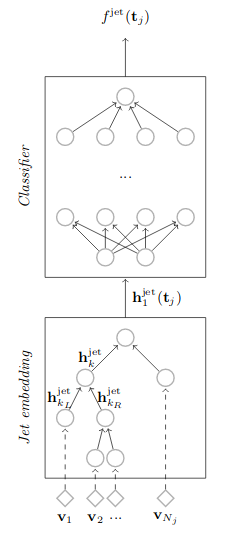
\includegraphics[width=0.2\textwidth]{Images/RecNN_architecture.png}
    \caption{Nodal architecture of a Recursive neural network (RecNN).}
    \label{fig:recnn_architecture}
\end{figure}

\begin{figure}
    \begin{center}
    \subfloat[RecNN leaf node]{
        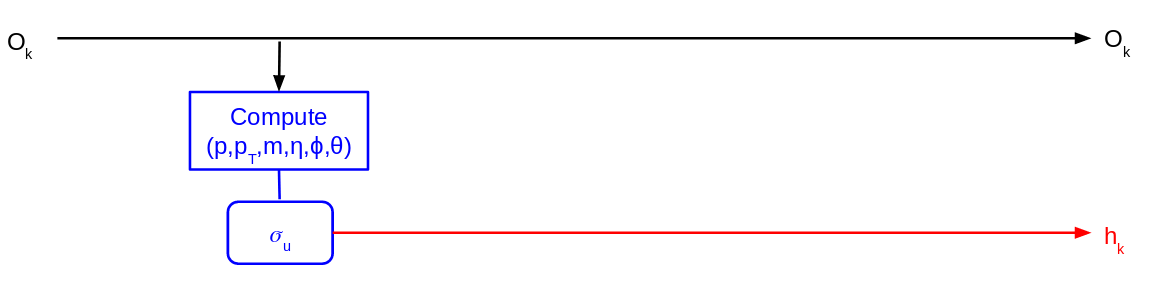
\includegraphics[width=\textwidth]{Images/simpleRecNN.png}
        \label{sub:RecNNLeafNode}
    }
    
    \subfloat[RecNN node]{
        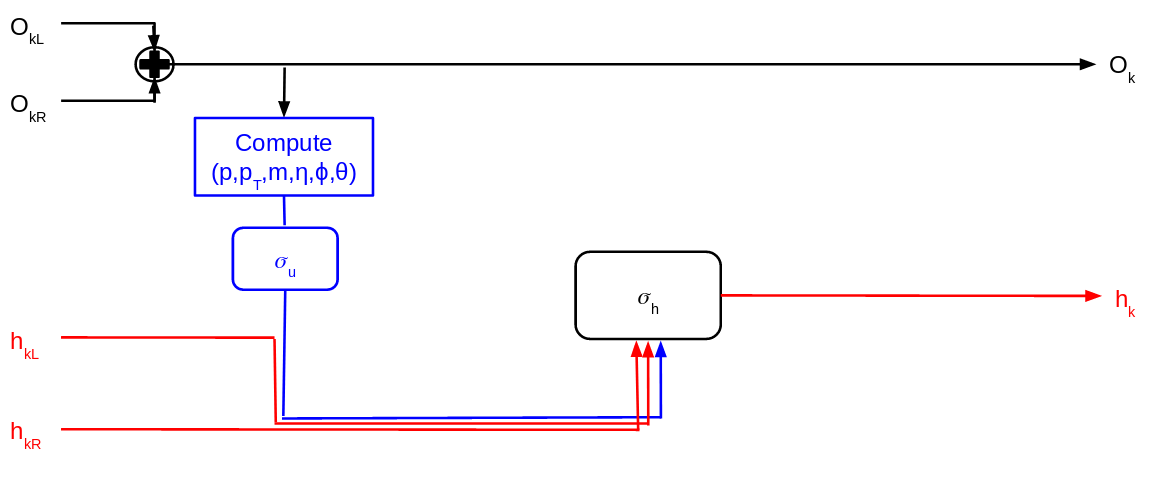
\includegraphics[width=\textwidth]{Images/simpleRecNN2.png}
        \label{sub:RecNNNode}
    }
    
    \subfloat[Gated RecNN node]{
        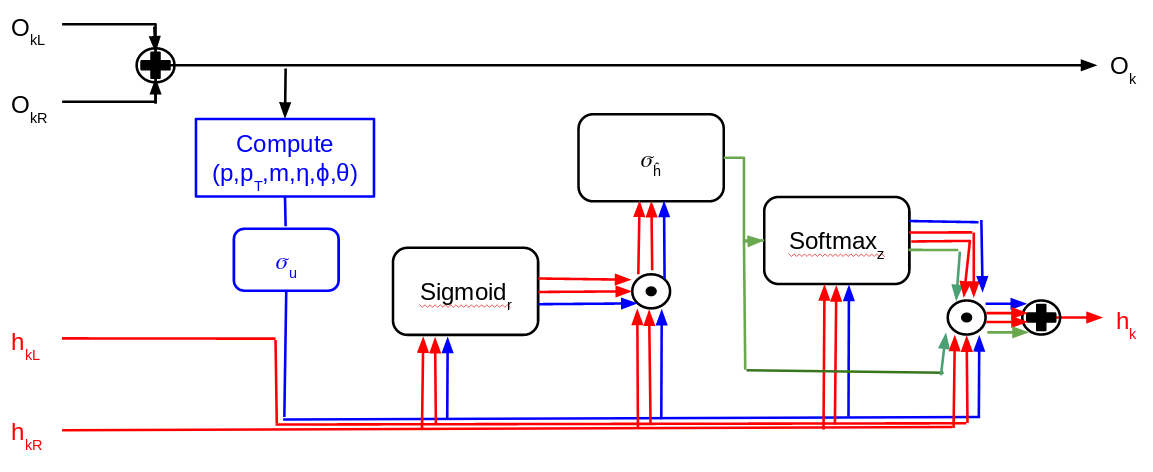
\includegraphics[width=\textwidth]{Images/gatedRecNN.png}
        \label{sub:GatedRecNNNode}
    }
    
    \caption{Diagrams of different nodes that can be found in a RecNN architectures. Top is a leaf node, middle is a non-leaf node. Bottom is a non-leaf node for a gated RecNN architecture.}
    \label{fig:recnn_nodes}
    \end{center}
\end{figure}

The network architecture will be divided into two parts : a first "jet embedding part" which will follow the jet clustering structure, which output will then be given as input to a dense feed-forward network architecture, see \ref{fig:recnn_architecture}.
The jet-embedding is an ensemble of nodes. Each set of particle variables is fed at its leaf-nodes, meaning each leaf-node will hold the defining characteristics of its associated particle. Then each node output will be merged with another node output in a new node. 
This is then a recursive process : from a list of nodes, two nodes are picked from a metric and merged, and so on until there is only one node.
The metric used to select which nodes are to be merged next can be selected among the following set:
    
\begin{itemize}
    \item randomized : two nodes are selected at random
    \item pt-ordered : the nodes holding the two pseudo-particles with the highest pt 
    \item reversed pt-ordered : the nodes holding the two pseudo-particles with the lowest pt
    \item kt : nodes holding closest pseudo-particles following the kt clustering metric
    \item cambridge : nodes holding closest pseudo-particles following the cambridge clustering metric
    \item anti-kt : nodes holding closest pseudo-particles following the anti-kt metric
\end{itemize}

This clustering scheme is going to be the base for two communicating paths taken by information, as figure \ref{fig:recnn_nodes} shows the path of information in the different types of nodes.
The vector $O_k$ was in previous work only the 4-momentum of the particle or pseudo-particle at the noke k. We have added the extra information of the energy part contribution by particle id : $E_{\gamma}$, $E_{e}$, $E_{\mu}$, $E_{h^{\pm}}$ and $E_{h^{0}}$. This should allow the network to base its decision on types of particles at every step. 
At each node a full set of variables is re-computed from the 4-momentum : p, \pt, m, $\eta$, $\phi$, $\theta$. All those variables are then fed into a neuron layer called $\sigma_{u}$.
On a leaf node k, the output of $\sigma_{u}$ is then taken as the embedded output of this node, named $h_k$.
On a non-leaf node k, the output of $\sigma_{u}$ is fed along the embedded outputs of the previous layers into another layer, namely $\sigma_h$. the output of $\sigma_h$ is then the embedded output $h_k$.
Effectively there are indeed two paths for the information in the architecture: a direct pseudo-particle like clustering where effective 4-momentum are added, and a path where neuron layers embed the information and mixes it with the existing previously embedded information.

\subsection{Gating}

Gated RecNN adds an extra complexity on the scheme of layers in a node, detailed in figure \ref{fig:recnn_nodes}. The gating is inspired by the long short-term memory (LSTM) architecture. It adds the possibility for the network to select and mix information in the embedding scheme more easily. 

A new neuron layer $Sigmoid_r$, takes 3 input vectors : $h_k_l$,$h_k_r$ and the output of layer $\sigma_u$. It will give 3 scalar outputs that will be used to multiply the same vectors respectively. Each multiplied vector is then fed into layer $\sigma_\hat{h}$. 
The four vectors $h_k_l$, $h_k_r$, output of $\sigma_u$ and output of $\sigma_\hat{h}$ are going to be weighted and added. The weights $w_i$ are given by another neuron layer. They respect the following equations :
\begin{equation}    
    h_{k} = \sum_{n_{i}=h_{kL},h_{kR},u,\hat{h}} w_{i}n_{i}
\end{equation}
\begin{equation}
    w_{i} = \frac{e^{Z_i}}{\sum_{j=1}^{K}e^{Z_j}}
\end{equation}
This will allow the network to easily enhance the importance of certain information paths and belittle information that it can deem to be not useful.

\subsection{Unbiasing the training sample}

jet centered and de-boosted, orientated.
all raw variables are scaled (sklearn.preprocessing.Robustscaler) before being fed into the network to avoid scaling issues

\begin{itemize}
    \item To first avoid biases, the number of signal and background "jets" are forced to be the same:
    \item in our case, having many more background "jets" at hand than signal "jets", every signal "jet" is kept and background is then selected
    \item This selection of background "jet" is not completely random, as in order to avoid biases in the training, pt distribution of background and signal must match.
    \item To achieve this, "jets" in the background samples are chosen at random, then are only added to the training sample if the number of background "jets" already selected in a given pt range is lower than the number of signal "jets" in the same pt range
\end{itemize}

\subsection{Performance}

\begin{figure}
    \centering
    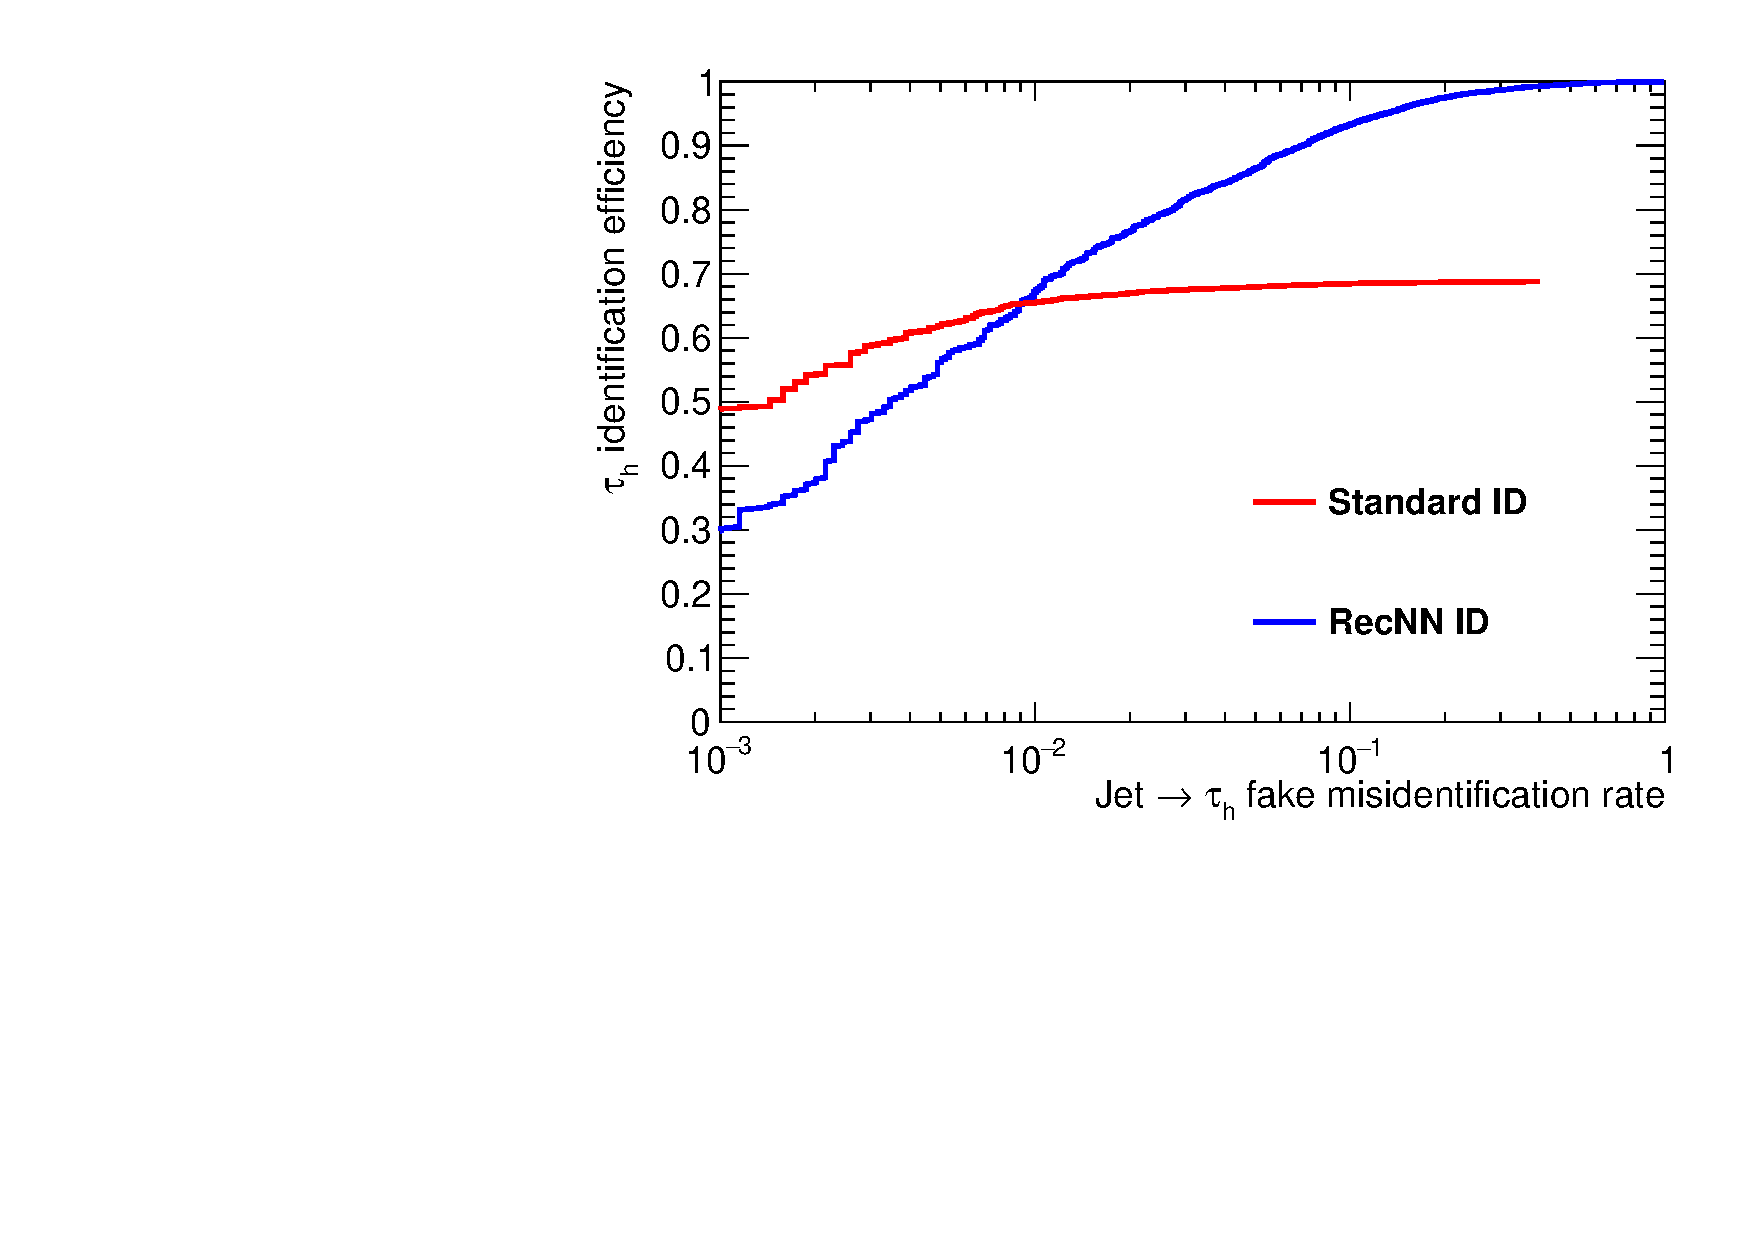
\includegraphics[width=\textwidth]{Images/RecNN_ROC.pdf}
    \caption{\tauh identification ROC curve for the standard method and with a RecNN.}
    \label{fig:RecNN_ROC}
\end{figure}

\begin{itemize}
    \item show all the plots
    \item so far all ordering are similar
    \item gated gives the best results
\end{itemize}

\subsection{Possible optimisation}

This section is on work that is not done yet ...

\begin{itemize}
    \item TODO, optimise the different inner layers (add more layers with more neurons = hyper-parameter optimisation)
    \item pre-train "embedding" layers following auto-encoder philosophy
    \item have subtrainings with subsets 
\end{itemize}
